\documentclass[twoside]{book}

% Packages required by doxygen
\usepackage{fixltx2e}
\usepackage{calc}
\usepackage{doxygen}
\usepackage[export]{adjustbox} % also loads graphicx
\usepackage{graphicx}
\usepackage[utf8]{inputenc}
\usepackage{makeidx}
\usepackage{multicol}
\usepackage{multirow}
\PassOptionsToPackage{warn}{textcomp}
\usepackage{textcomp}
\usepackage[nointegrals]{wasysym}
\usepackage[table]{xcolor}

% Font selection
\usepackage[T1]{fontenc}
\usepackage[scaled=.90]{helvet}
\usepackage{courier}
\usepackage{amssymb}
\usepackage{sectsty}
\renewcommand{\familydefault}{\sfdefault}
\allsectionsfont{%
  \fontseries{bc}\selectfont%
  \color{darkgray}%
}
\renewcommand{\DoxyLabelFont}{%
  \fontseries{bc}\selectfont%
  \color{darkgray}%
}
\newcommand{\+}{\discretionary{\mbox{\scriptsize$\hookleftarrow$}}{}{}}

% Page & text layout
\usepackage{geometry}
\geometry{%
  a4paper,%
  top=2.5cm,%
  bottom=2.5cm,%
  left=2.5cm,%
  right=2.5cm%
}
\tolerance=750
\hfuzz=15pt
\hbadness=750
\setlength{\emergencystretch}{15pt}
\setlength{\parindent}{0cm}
\setlength{\parskip}{3ex plus 2ex minus 2ex}
\makeatletter
\renewcommand{\paragraph}{%
  \@startsection{paragraph}{4}{0ex}{-1.0ex}{1.0ex}{%
    \normalfont\normalsize\bfseries\SS@parafont%
  }%
}
\renewcommand{\subparagraph}{%
  \@startsection{subparagraph}{5}{0ex}{-1.0ex}{1.0ex}{%
    \normalfont\normalsize\bfseries\SS@subparafont%
  }%
}
\makeatother

% Headers & footers
\usepackage{fancyhdr}
\pagestyle{fancyplain}
\fancyhead[LE]{\fancyplain{}{\bfseries\thepage}}
\fancyhead[CE]{\fancyplain{}{}}
\fancyhead[RE]{\fancyplain{}{\bfseries\leftmark}}
\fancyhead[LO]{\fancyplain{}{\bfseries\rightmark}}
\fancyhead[CO]{\fancyplain{}{}}
\fancyhead[RO]{\fancyplain{}{\bfseries\thepage}}
\fancyfoot[LE]{\fancyplain{}{}}
\fancyfoot[CE]{\fancyplain{}{}}
\fancyfoot[RE]{\fancyplain{}{\bfseries\scriptsize Generated by Doxygen }}
\fancyfoot[LO]{\fancyplain{}{\bfseries\scriptsize Generated by Doxygen }}
\fancyfoot[CO]{\fancyplain{}{}}
\fancyfoot[RO]{\fancyplain{}{}}
\renewcommand{\footrulewidth}{0.4pt}
\renewcommand{\chaptermark}[1]{%
  \markboth{#1}{}%
}
\renewcommand{\sectionmark}[1]{%
  \markright{\thesection\ #1}%
}

% Indices & bibliography
\usepackage{natbib}
\usepackage[titles]{tocloft}
\setcounter{tocdepth}{3}
\setcounter{secnumdepth}{5}
\makeindex

% Hyperlinks (required, but should be loaded last)
\usepackage{ifpdf}
\ifpdf
  \usepackage[pdftex,pagebackref=true]{hyperref}
\else
  \usepackage[ps2pdf,pagebackref=true]{hyperref}
\fi
\hypersetup{%
  colorlinks=true,%
  linkcolor=blue,%
  citecolor=blue,%
  unicode%
}

% Custom commands
\newcommand{\clearemptydoublepage}{%
  \newpage{\pagestyle{empty}\cleardoublepage}%
}

\usepackage{caption}
\captionsetup{labelsep=space,justification=centering,font={bf},singlelinecheck=off,skip=4pt,position=top}

%===== C O N T E N T S =====

\begin{document}

% Titlepage & ToC
\hypersetup{pageanchor=false,
             bookmarksnumbered=true,
             pdfencoding=unicode
            }
\pagenumbering{alph}
\begin{titlepage}
\vspace*{7cm}
\begin{center}%
{\Large Computer\+\_\+\+Homework2 }\\
\vspace*{1cm}
{\large Generated by Doxygen 1.8.13}\\
\end{center}
\end{titlepage}
\clearemptydoublepage
\pagenumbering{roman}
\tableofcontents
\clearemptydoublepage
\pagenumbering{arabic}
\hypersetup{pageanchor=true}

%--- Begin generated contents ---
\chapter{File Index}
\section{File List}
Here is a list of all documented files with brief descriptions\+:\begin{DoxyCompactList}
\item\contentsline{section}{/home/lis1331/\+Documents/lecture/phy/computer/comp\+\_\+hw/\+H\+W3/src/\hyperlink{hw3_8cpp}{hw3.\+cpp} \\*Code for homework3 of Computer1 class in Yonsei University Minimize the action by Markov Chain Monte Carlo Method to solve Kepler problem }{\pageref{hw3_8cpp}}{}
\item\contentsline{section}{/home/lis1331/\+Documents/lecture/phy/computer/comp\+\_\+hw/\+H\+W3/src/\hyperlink{main_8cpp}{main.\+cpp} \\*Main program for homework3 of Computer1 class in Yonsei University Interactively reads inital condition, number of sine function used for guess, number of gird points to evaluate, number of interation, step size and output file name then computes and saves solution }{\pageref{main_8cpp}}{}
\item\contentsline{section}{/home/lis1331/\+Documents/lecture/phy/computer/comp\+\_\+hw/\+H\+W3/src/\hyperlink{support_8cpp}{support.\+cpp} \\*Support functions for homework3 of Computer1 class in Yonsei University scale and add vector, evaluate sum and derivative of sine function, randomly move initial guess by step and evaluate the action of given path }{\pageref{support_8cpp}}{}
\item\contentsline{section}{/home/lis1331/\+Documents/lecture/phy/computer/comp\+\_\+hw/\+H\+W3/src/include/\hyperlink{hw3_8hpp}{hw3.\+hpp} \\*Headerfile for homework3 of Computer1 class in Yonsei University Minimize the action by Markov Chain Monte Carlo Method to solve Kepler problem }{\pageref{hw3_8hpp}}{}
\end{DoxyCompactList}

\chapter{File Documentation}
\hypertarget{hw2_8cpp}{}\section{/home/lis1331/\+Documents/lecture/phy/computer/comp\+\_\+hw/\+H\+W2/src/hw2.cpp File Reference}
\label{hw2_8cpp}\index{/home/lis1331/\+Documents/lecture/phy/computer/comp\+\_\+hw/\+H\+W2/src/hw2.\+cpp@{/home/lis1331/\+Documents/lecture/phy/computer/comp\+\_\+hw/\+H\+W2/src/hw2.\+cpp}}


code for homework2 of Computer1 class in Yonsei University Use numerical integration to solve Kepler problem  


{\ttfamily \#include \char`\"{}hw2.\+hpp\char`\"{}}\newline
Include dependency graph for hw2.\+cpp\+:
\nopagebreak
\begin{figure}[H]
\begin{center}
\leavevmode
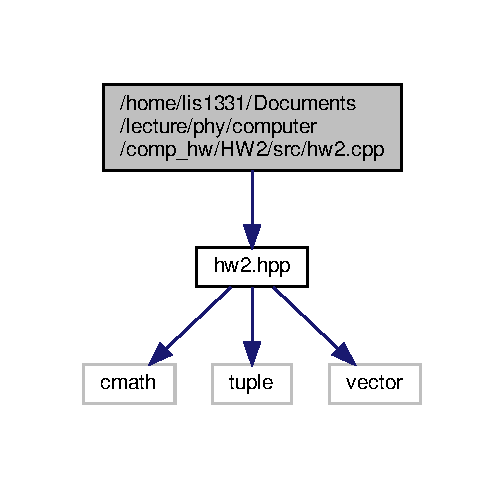
\includegraphics[width=242pt]{hw2_8cpp__incl}
\end{center}
\end{figure}
\subsection*{Functions}
\begin{DoxyCompactItemize}
\item 
tuple$<$ vector$<$ double $>$, vector$<$ double $>$ $>$ \hyperlink{hw2_8cpp_a4beb2c3e1dbd86eaed9e661ee19afbcc}{H\+W2} (double zeta\+\_\+min, double t0, int n)
\begin{DoxyCompactList}\small\item\em H\+W2\+: Solve Kepler problem via numerical integration from zeta\+\_\+min to zeta\+\_\+max see H\+W2.\+pdf for further detail. \end{DoxyCompactList}\end{DoxyCompactItemize}


\subsection{Detailed Description}
code for homework2 of Computer1 class in Yonsei University Use numerical integration to solve Kepler problem 

\begin{DoxyAuthor}{Author}
pistack (Junho Lee) 
\end{DoxyAuthor}
\begin{DoxyDate}{Date}
2021. 10. 10. 
\end{DoxyDate}


\subsection{Function Documentation}
\mbox{\Hypertarget{hw2_8cpp_a4beb2c3e1dbd86eaed9e661ee19afbcc}\label{hw2_8cpp_a4beb2c3e1dbd86eaed9e661ee19afbcc}} 
\index{hw2.\+cpp@{hw2.\+cpp}!H\+W2@{H\+W2}}
\index{H\+W2@{H\+W2}!hw2.\+cpp@{hw2.\+cpp}}
\subsubsection{\texorpdfstring{H\+W2()}{HW2()}}
{\footnotesize\ttfamily tuple$<$vector$<$double$>$, vector$<$double$>$ $>$ H\+W2 (\begin{DoxyParamCaption}\item[{double}]{zeta\+\_\+min,  }\item[{double}]{t0,  }\item[{int}]{n }\end{DoxyParamCaption})}



H\+W2\+: Solve Kepler problem via numerical integration from zeta\+\_\+min to zeta\+\_\+max see H\+W2.\+pdf for further detail. 


\begin{DoxyParams}{Parameters}
{\em zeta\+\_\+min} & minimum value of zeta, for constraint motion 0.\+5 $<$ zeta\+\_\+min $<$ 1 \\
\hline
{\em t0} & initial time \\
\hline
{\em n} & number of points to evaluate \\
\hline
\end{DoxyParams}
\begin{DoxyReturn}{Returns}
tuple of time and zeta 
\end{DoxyReturn}

\hypertarget{hw2_8hpp}{}\section{/home/lis1331/\+Documents/lecture/phy/computer/comp\+\_\+hw/\+H\+W2/src/include/hw2.hpp File Reference}
\label{hw2_8hpp}\index{/home/lis1331/\+Documents/lecture/phy/computer/comp\+\_\+hw/\+H\+W2/src/include/hw2.\+hpp@{/home/lis1331/\+Documents/lecture/phy/computer/comp\+\_\+hw/\+H\+W2/src/include/hw2.\+hpp}}


headerfile for homework2 of Computer1 class in Yonsei University Use numerical integration to solve Kepler problem  


{\ttfamily \#include $<$cmath$>$}\newline
{\ttfamily \#include $<$tuple$>$}\newline
{\ttfamily \#include $<$vector$>$}\newline
Include dependency graph for hw2.\+hpp\+:
\nopagebreak
\begin{figure}[H]
\begin{center}
\leavevmode
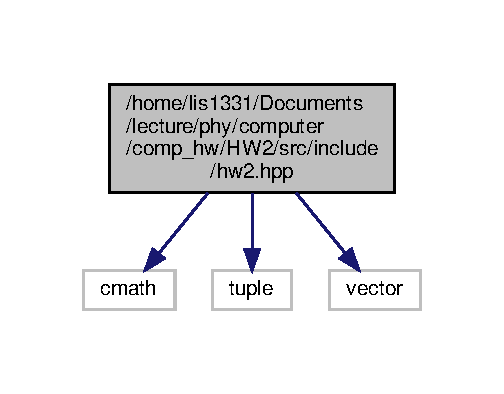
\includegraphics[width=242pt]{hw2_8hpp__incl}
\end{center}
\end{figure}
This graph shows which files directly or indirectly include this file\+:
\nopagebreak
\begin{figure}[H]
\begin{center}
\leavevmode
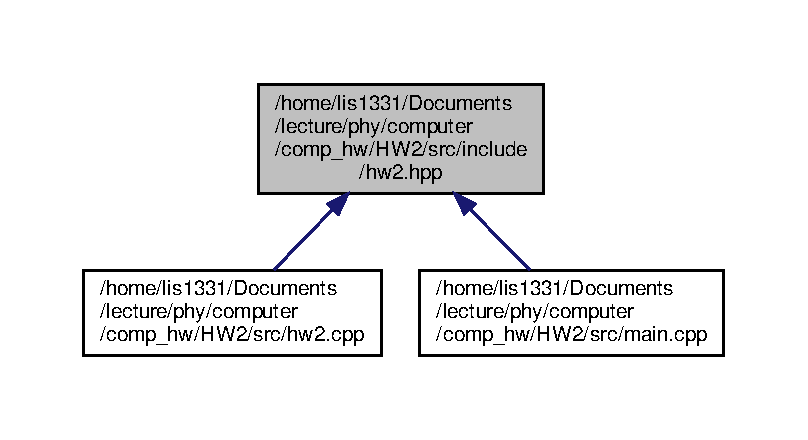
\includegraphics[width=350pt]{hw2_8hpp__dep__incl}
\end{center}
\end{figure}
\subsection*{Functions}
\begin{DoxyCompactItemize}
\item 
std\+::tuple$<$ std\+::vector$<$ double $>$, std\+::vector$<$ double $>$ $>$ \hyperlink{hw2_8hpp_aef3f570bcb6b0cff581234630db4a551}{H\+W2} (double zeta\+\_\+min, double t0, int n)
\begin{DoxyCompactList}\small\item\em H\+W2\+: Solve Kepler problem via numerical integration from zeta\+\_\+min to zeta\+\_\+max see H\+W2.\+pdf for further detail. \end{DoxyCompactList}\end{DoxyCompactItemize}


\subsection{Detailed Description}
headerfile for homework2 of Computer1 class in Yonsei University Use numerical integration to solve Kepler problem 

\begin{DoxyAuthor}{Author}
pistack (Junho Lee) 
\end{DoxyAuthor}
\begin{DoxyDate}{Date}
2021. 10. 10. 
\end{DoxyDate}


\subsection{Function Documentation}
\mbox{\Hypertarget{hw2_8hpp_aef3f570bcb6b0cff581234630db4a551}\label{hw2_8hpp_aef3f570bcb6b0cff581234630db4a551}} 
\index{hw2.\+hpp@{hw2.\+hpp}!H\+W2@{H\+W2}}
\index{H\+W2@{H\+W2}!hw2.\+hpp@{hw2.\+hpp}}
\subsubsection{\texorpdfstring{H\+W2()}{HW2()}}
{\footnotesize\ttfamily std\+::tuple$<$std\+::vector$<$double$>$, std\+::vector$<$double$>$ $>$ H\+W2 (\begin{DoxyParamCaption}\item[{double}]{zeta\+\_\+min,  }\item[{double}]{t0,  }\item[{int}]{n }\end{DoxyParamCaption})}



H\+W2\+: Solve Kepler problem via numerical integration from zeta\+\_\+min to zeta\+\_\+max see H\+W2.\+pdf for further detail. 


\begin{DoxyParams}{Parameters}
{\em zeta\+\_\+min} & minimum value of zeta, for constraint motion 0.\+5 $<$ zeta\+\_\+min $<$ 1 \\
\hline
{\em t0} & initial time \\
\hline
{\em n} & number of points to evaluate \\
\hline
\end{DoxyParams}
\begin{DoxyReturn}{Returns}
tuple of time and zeta 
\end{DoxyReturn}

\hypertarget{main_8cpp}{}\section{/home/lis1331/\+Documents/lecture/phy/computer/comp\+\_\+hw/\+H\+W3/src/main.cpp File Reference}
\label{main_8cpp}\index{/home/lis1331/\+Documents/lecture/phy/computer/comp\+\_\+hw/\+H\+W3/src/main.\+cpp@{/home/lis1331/\+Documents/lecture/phy/computer/comp\+\_\+hw/\+H\+W3/src/main.\+cpp}}


main program for homework3 of Computer1 class in Yonsei University Interactively reads inital condition, number of sine function used for guess, number of gird points to evaluate, number of interation, step size and output file name then computes and saves solution.  


{\ttfamily \#include $<$string$>$}\newline
{\ttfamily \#include $<$iostream$>$}\newline
{\ttfamily \#include $<$fstream$>$}\newline
{\ttfamily \#include \char`\"{}hw3.\+hpp\char`\"{}}\newline
Include dependency graph for main.\+cpp\+:\nopagebreak
\begin{figure}[H]
\begin{center}
\leavevmode
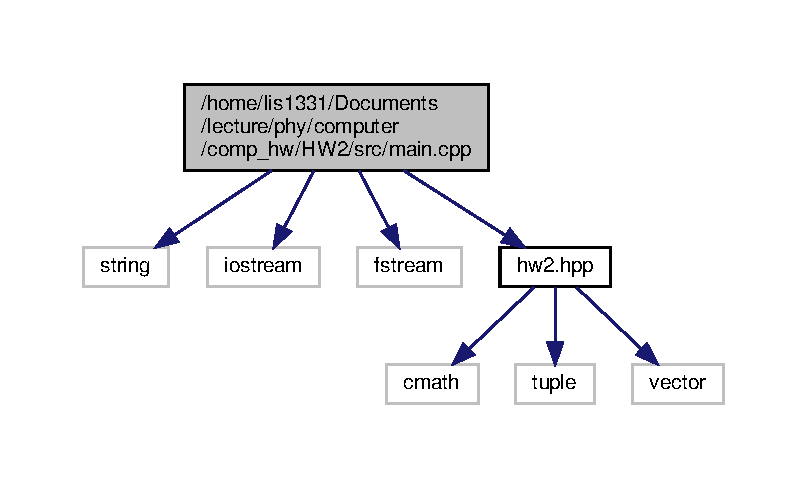
\includegraphics[width=350pt]{main_8cpp__incl}
\end{center}
\end{figure}
\subsection*{Functions}
\begin{DoxyCompactItemize}
\item 
\mbox{\Hypertarget{main_8cpp_a840291bc02cba5474a4cb46a9b9566fe}\label{main_8cpp_a840291bc02cba5474a4cb46a9b9566fe}} 
int {\bfseries main} (void)
\end{DoxyCompactItemize}


\subsection{Detailed Description}
main program for homework3 of Computer1 class in Yonsei University Interactively reads inital condition, number of sine function used for guess, number of gird points to evaluate, number of interation, step size and output file name then computes and saves solution. 

\begin{DoxyAuthor}{Author}
pistack (Junho Lee) 
\end{DoxyAuthor}
\begin{DoxyDate}{Date}
2021. 10. 10. 
\end{DoxyDate}

%--- End generated contents ---

% Index
\backmatter
\newpage
\phantomsection
\clearemptydoublepage
\addcontentsline{toc}{chapter}{Index}
\printindex

\end{document}
